\chapter{Sensor fusion and SLAM} \label{ch:slam}

SLAM consists of simultaneous estimation of the state of a robot equipped with onboard sensors, and the construction of a map of the environment that the sensors are perceiving \citep{slamtut2006part1}. The robot state is often described by its pose (position and orientation), although other quantities may be included. The map represents aspects of interest (e.g. obstacles) describing the robot's surrounding environment. Both of these things, the robot pose and a map of the surroundings, are critical components for tasks such as path planning. Consequently, SLAM is often a key component in autonomous operations where a prior map of the environment is not available.

SLAM systems require some sort of mapping data about their surrounding environment. This data can come from sensors such as lidar \citep{cartographerPaper}, sonar \citep{norgren2018multibeam}, or camera \citep{orbslam2017} (often called visual SLAM or VSLAM). In order to increase reliability and robustness, most SLAM systems also support input from other types of sensors such as IMU, different types of odometry (e.g. wheel odometry for wheeled robots), altimeter for aerial vehicles, or GNSS \citep{website:Cartographer,hector2011slam}. As a result, SLAM is a valuable tool for sensor fusion. 

In this chapter, the sensors of the Otter USV are presented together with the drivers required to get the sensor data into ROS. The chapter also takes a closer look how the data from the sensors are used, and why the sensors are needed. Finally, the SLAM system Cartographer \citep{cartographerPaper} is set up for real-time 2D SLAM in ROS.

\section{Sensors and drivers}

\subsection{Lidar}

In this thesis, mapping of the surrounding environment is done with the RPLIDAR A3 \citep{website:rplidara3}, a low-cost 2D lidar. The lidar states a range of 25 m, 360-degree field of view, 16000 samples per second, and outdoor availability. A ready-to-use ROS driver, the \path{rplidar_ros} package \citep{website:rplidarDriver}, provides the system with \path{sensor_msgs/LaserScan} messages. This is a data type which holds an array of ranges and their corresponding angles for one complete revolution of the lidar. The lidar and a visualization of a laser scan is shown in \figref{fig:lidar_sensor}.

\begin{figure}[h!]
    \centering
	\makebox[\linewidth][c]{
	\begin{subfigure}[b]{0.5\textwidth}
		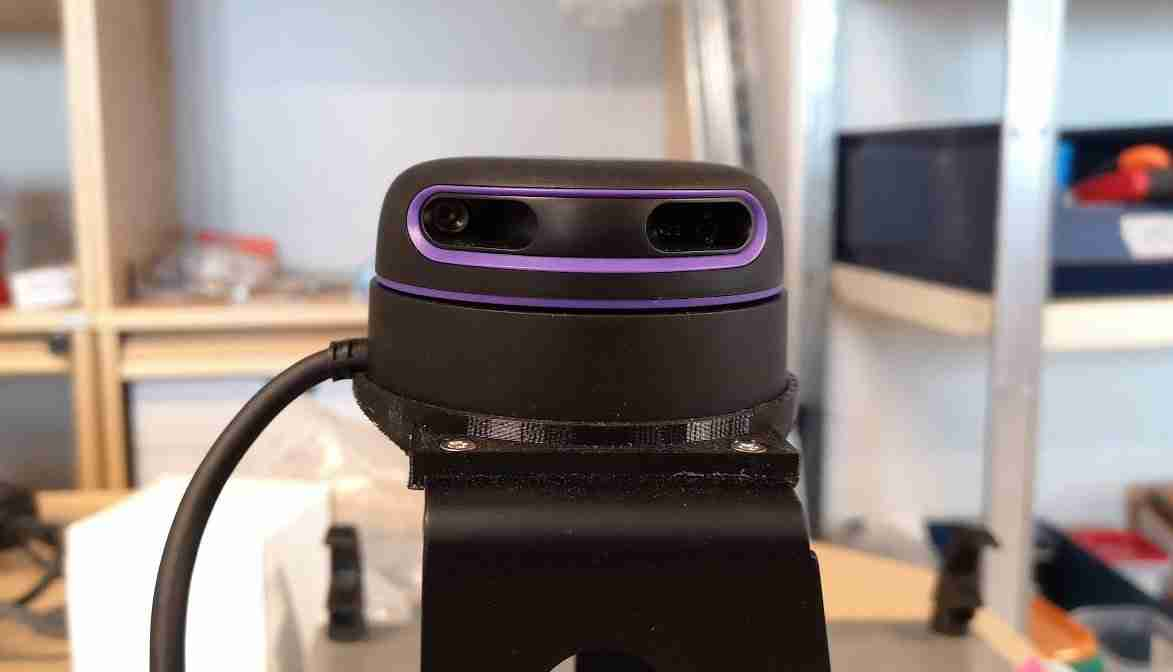
\includegraphics[width=1\linewidth]{fig/instrumentation/rplidara31}
		\caption{}
	\end{subfigure}
	\begin{subfigure}[b]{0.5\textwidth}
		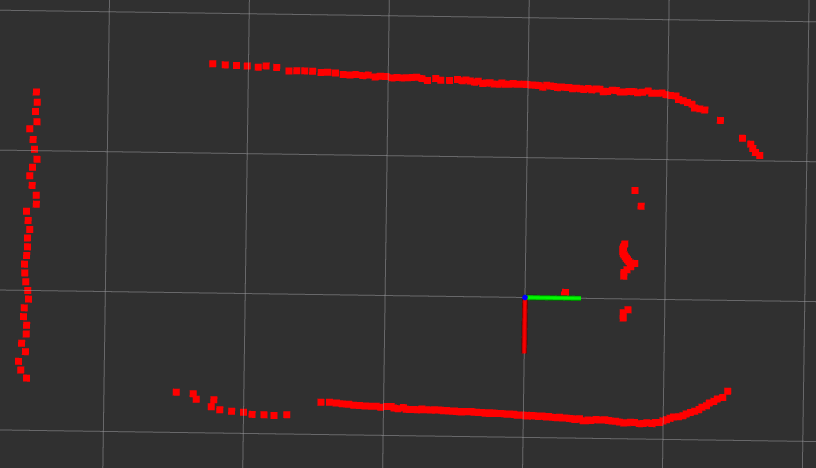
\includegraphics[width=1\linewidth]{fig/instrumentation/lidar_scan}
		\caption{}
	\end{subfigure}
	}
	\caption[The RPLIDAR A3]{(a) The RPLIDAR A3. (b) A lidar scan of a small room. The red, green and blue axis is the position of the lidar} \label{fig:lidar_sensor}
\end{figure}

It is possible to autonomously navigate a USV with only a lidar and SLAM, see for instance \citet{Ueland2016}. However, this requires a feature-rich environment in which it is always possible to find and recognize distinct features between subsequent lidar scans. Consequently, autonomous navigation with only a lidar is not feasible for situations where distances to the nearest obstacles often exceeds the range of the lidar. Additional sensors are also required in scenarios where the lidar is not able to see any difference in the environment between two consecutive poses, e.g. in a long corridor or while following a long uniform wall or edge. Since scenarios such as these are likely to be common in a typical application of the complete system, additional sensors are required.

\subsection{IMU}

Supplementing the lidar with an IMU increases the robustness and reliability of the sensing. This is because the IMU provides accurate orientation, rotational velocity, and linear acceleration, which can be used as initial estimates for the USV pose when comparing subsequent lidar scans in SLAM. This is especially useful for a USV operating on the water surface, since roll and pitch motions are otherwise hard to compensate for. The implemented system uses an AHRS of the type Xsens MTi \citep{website:xsens}, see \figref{fig:xsens}. The Xsens MTi comes with a ROS driver, the \path{xsens_driver} package \citep{website:xsensDriver}. This driver provides ROS with \path{sensor_msgs/Imu} messages, which contain orientation, angular velocity, and linear acceleration. The Xsens, being an AHRS, reports orientation relative to magnetic north, and the magnetic declination of the operating area can be looked up (e.g. at \citet{website:magcalc}). Having the orientation relative to true north makes it possible to later combine the IMU data with for example GNSS data.

%Thus, true heading is available to the system and can be used to translate angles in the SLAM map to course angle assignments.

\begin{figure}[h!]
	\centering
	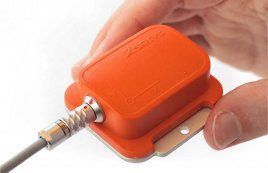
\includegraphics[width=0.5\linewidth]{fig/instrumentation/xsens_mti2}
	\caption[The Xsens MTi.]{The Xsens MTi AHRS, courtesy of Xsens.}
	\label{fig:xsens}
\end{figure}

\subsection{GNSS}

The combination of lidar and IMU works very well in many situations. SLAM systems usually have no problem localizing and generating maps when there are many objects within the range of the lidar. However, consider scenarios such as in \figref{fig:lidar_gnss} where the lidar detects nothing at all or too little for accurate localization. Based only on the detections generated from \figref{fig:lidar_gnss}b, the USV can be at any point along the wall. In situations such as these, the SLAM system is mostly relying on IMU data for positioning, and position estimates based on integration of linear accelerations from an IMU will quickly drift. For the intended purposes of the implemented system, scenarios such as these are to be expected. Thus, another form of positioning is needed, and in this case GNSS is used.

\begin{figure}[h!]
    \centering
	\makebox[\linewidth][c]{
	\begin{subfigure}[b]{0.5\textwidth}
		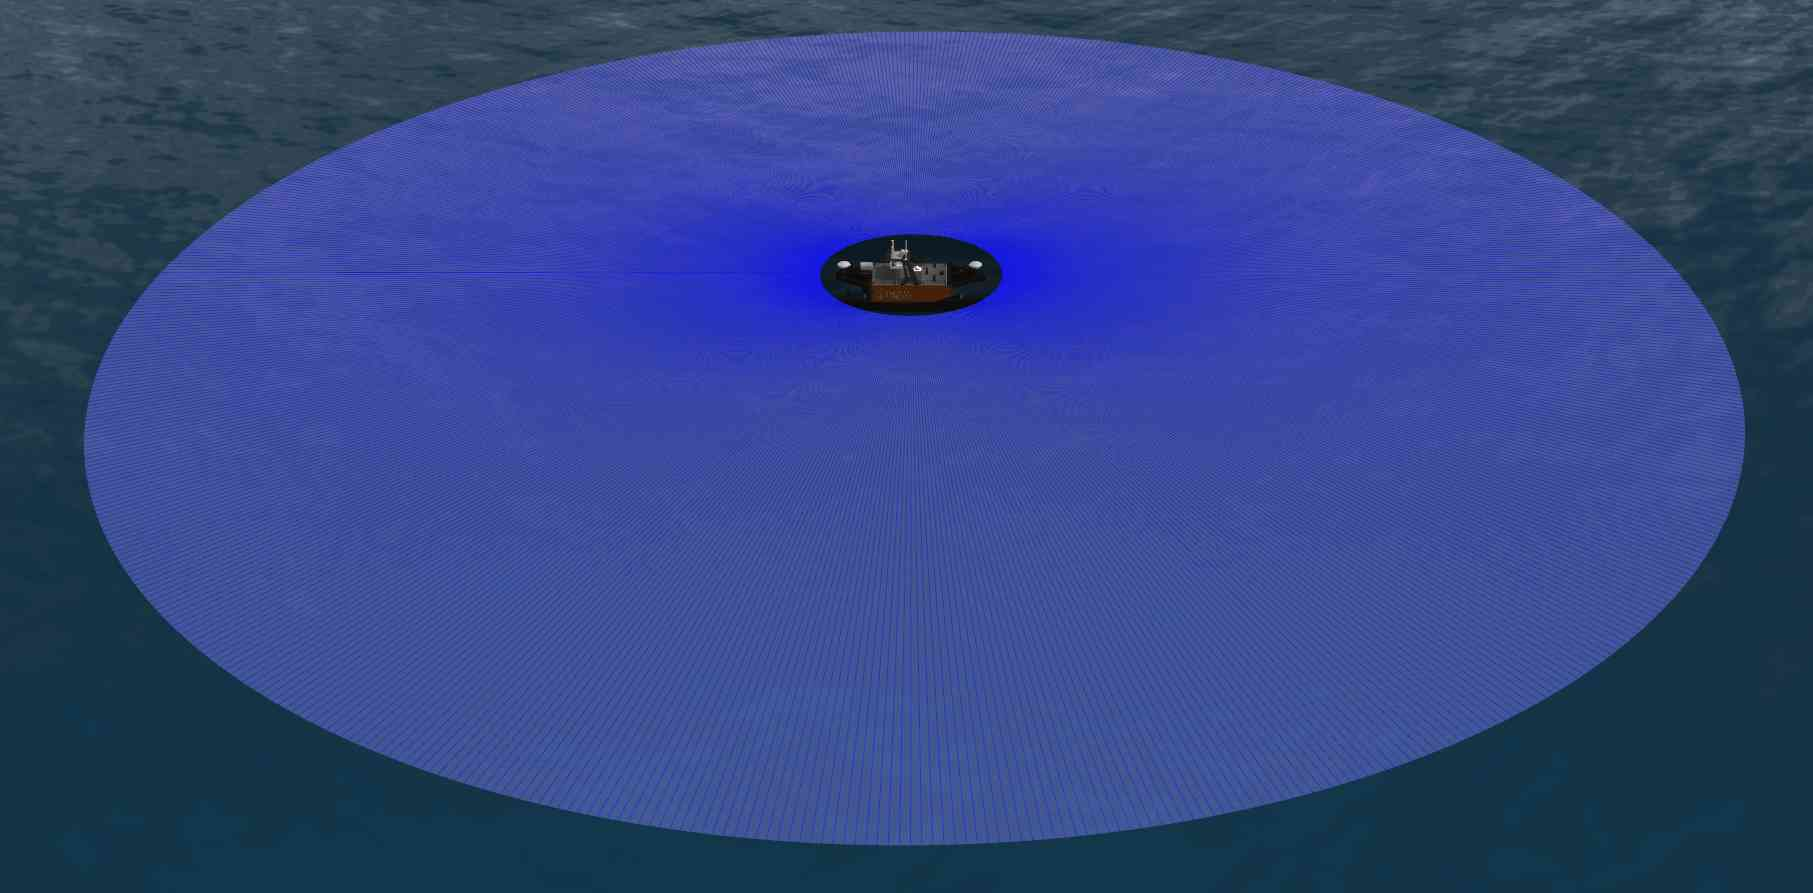
\includegraphics[width=1\linewidth]{fig/instrumentation/lidar_nothing.jpg}
		\caption{}
	\end{subfigure}
	\begin{subfigure}[b]{0.5\textwidth}
		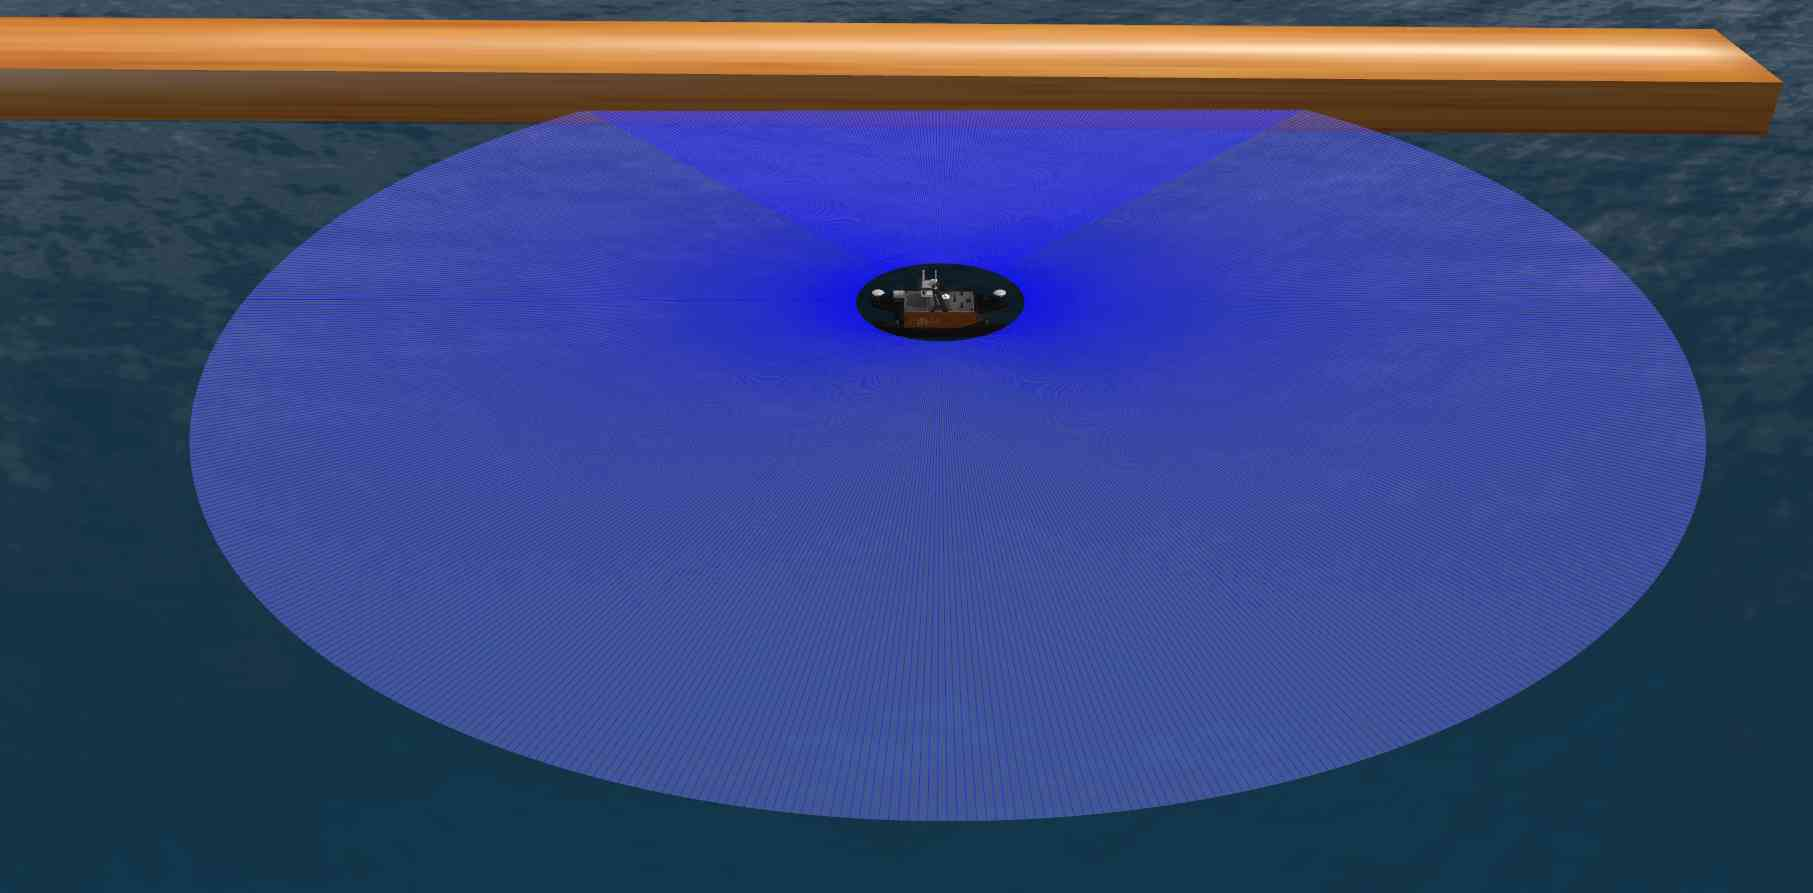
\includegraphics[width=1\linewidth]{fig/instrumentation/lidar_only_wall.jpg}
		\caption{}
	\end{subfigure}
	}
	\caption[Lidar detects nothing or too little for accurate localization.]{(a) No obstacles are within the lidar range. (b) The section of the wall within the lidar range does not provide enough information for localization.} \label{fig:lidar_gnss}
\end{figure}

The GNSS receiver on the USV reports its position as NMEA 0183 GGA messages. NMEA 0183 is a data specification standard for communication between marine electronics, defined by the National Marine Electronics Association \citep{wiki:nmea}. The GGA messages contain, most importantly, the latitude and longitude of the GNSS receiver. These messages are parsed with the \path{nmea_navsat_driver} ROS driver \citep{website:nmeaDriver}, which has been slightly modified to allow incoming NMEA messages over TCP. The driver provides the system with \path{sensor_msgs/NavSatFix} messages, which contain the latitude and longitude.

% The driver also provides the course angle $\chi$ as \code{geometry\_msgs/QuaternionStamped}.

\subsection{MBES}

The multibeam echosounder measures the depth in a fan shape beneath the USV. This data is not necessary for collision-free maneuvering on the surface, and is therefore not included in SLAM. There are SLAM systems that use MBES data (e.g. \citet{norgren2018multibeam}), so the MBES could potentially be included in SLAM in order to increase the accuracy. In this thesis, however, the MBES is only used for keeping track of the covered area and adapting the spacing between laps in the boustrophedon motions CCPP method. 

To use the MBES, the coverage range must be calculated. Let a detection point be described by the angle $\alpha$ relative to a line straight down from the USV, and let the reported distance for that angle be $f(\alpha)$, see \figref{fig:mbes_range}. Finding the detection point with the maximum angle $\alpha_{max}$ and minimum angle $\alpha_{min}$, it is then possible to find the coverage range in the port and starboard direction with
\begin{align}
c_p &= f(\alpha_{min}) \sin(\alpha_{min}) \\
c_s &= f(\alpha_{max}) \sin(\alpha_{max})
\end{align}
where $c_p$ and $c_s$ are the coverage ranges in port and starboard directions.

\begin{figure}[h!]
	\centering
	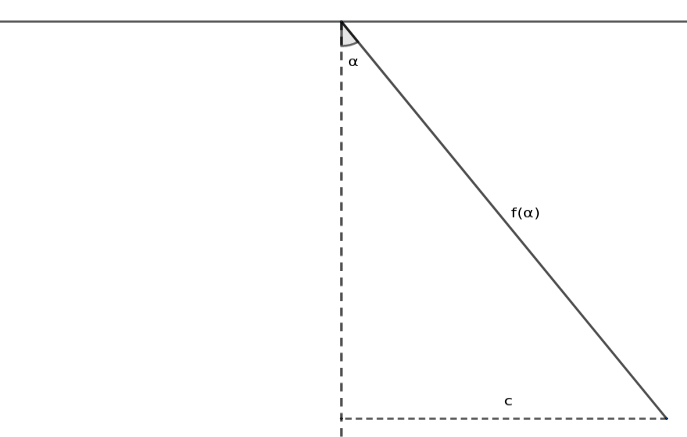
\includegraphics[width=0.5\linewidth]{fig/instrumentation/mbes_range2}
	\caption{Geometry of detection points of the MBES.}
	\label{fig:mbes_range}
\end{figure}

\section{SLAM with Cartographer}

Cartographer provides real-time SLAM in 2D and 3D across multiple platforms and sensor configurations \citep{website:Cartographer}. In this thesis, the ROS integration of Cartographer \citep{website:CartographerRos} is applied for 2D operation. By using the 2D version of Cartographer it is assumed that the floor (water surface) is flat, which is an okay assumption with a 2D lidar in sheltered waters. This only causes trouble if the heave motion of the USV causes the lidar to detect different things at different heights. The 2D version is chosen mainly because it is simpler to work with, as it requires fewer parameters to be tuned. Furthermore, the additional benefits of a 3D map are not required for the application in this thesis.

Out of the box, Cartographer accepts \path{sensor_msgs/LaserScan} and \path{sensor_msgs/Imu} messages from the lidar and IMU. However, the 2D version does not readily accept \path{sensor_msgs/NavSatFix} messages from the GNSS receiver. To get around this, it is possible to fuse data from the IMU and GNSS with an extended Kalman filter (EKF) in order to generate pose estimates as \path{nav_msgs/Odometry} messages. These messages can in turn be provided to Cartographer. The \path{robot_localization} package in ROS \citep{ros:robotlocalization} offers a collection of state estimation implementations for incorporation of GNSS data which has been used in this thesis. The information flow described in this chapter is illustrated in \figref{fig:sensor_fusion}.

\begin{figure}[h!]
	\centering
	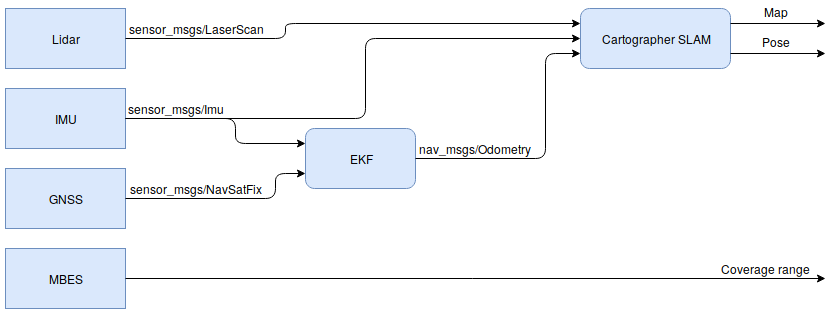
\includegraphics[width=1.0\linewidth]{fig/instrumentation/sensor_fusion}
	\caption{Information flow in sensor fusion and SLAM.}
	\label{fig:sensor_fusion}
\end{figure} 

Tuning Cartographer is difficult, as it is a very complex system where many of the parameters affect each other. A tuning methodology is provided by the authors at \citet{website:CartographerRos}. Tuning includes, among many other things, to set parameters for the scan matcher, the size and resolution of the submaps, and how much to trust odometry. For instance, since the provided odometry is a fusing of accurate IMU and GNSS data, it should be trusted with a high weight. The exact values to set is often a matter of experimenting and seeing what yields the best results. The parameters used in the experiments are provided in Appendix \ref{app:cartographer}.


